%\begin{frame}[fragile]{The expansion constant $c$}
%
%Given a metric space $X$ with distance $d : X \times X \to \mathbb{R}$, define
%\vspace{0.15in}
%
%\textbf{ball of radius $r$ centered at point $p$ }:
%$$
%B(p,r) = \{q \in X : d(p,q) \le r \}
%$$
%
%%\textbf{expansion constant $(c)$}: the smallest value $c \ge 2$ such that
%%$$
%%|B(p,2r)| \le c|B(p,r)|
%%$$
%%for every $p$ in the metric space $X$ and $r\ge0$.
%
%\textbf{expansion constant}:
%$$
%c = \sup_{p\in X, r\ge0} \left\{
    %\frac{|B(p,2r)|}{|B(p,r)|}
      %\right\}
%$$
%
%\hrule
%
%\vspace{0.15in}
%properties of the expansion constant:
%\begin{enumerate}
%\item dimension $(=\log c)$ of $\mathbb{R}^n$ is $O(n)$
%\item roughly captures the ``intrinsic dimensionality'' of $X$
%\item adding a single new point to $X$ can increase $c$ by an arbitrary amount;
%
%there are subsets of $\mathbb{R}^2$ with $c=\infty$
%\end{enumerate}
%
%\end{frame}

%%%%%%%%%%%%%%%%%%%%%%%%%%%%%%%%%%%%%%%%%%%%%%%%%%%%%%%%%%%%%%%%%%%%%%%%%%%%%%%%

\begin{frame}[fragile]{The expansion constant $\cexp$ is a type of dimension}

The \textbf{expansion constant} is defined as:
$$
\cexp = \sup_{p\in X, r\ge0} \left\{
    \frac{|B(p,2r)|}{|B(p,r)|}
      \right\}
$$
where
$$
B(p,r) = \{q \in X : d(p,q) \le r \}
$$
is the ball of radius $r$ centered at point $p$.
\vspace{0.15in}

\hrule
\vspace{0.15in}

\begin{tabular}{m{4cm}m{7cm} }
\resizebox{!}{3.5cm}{
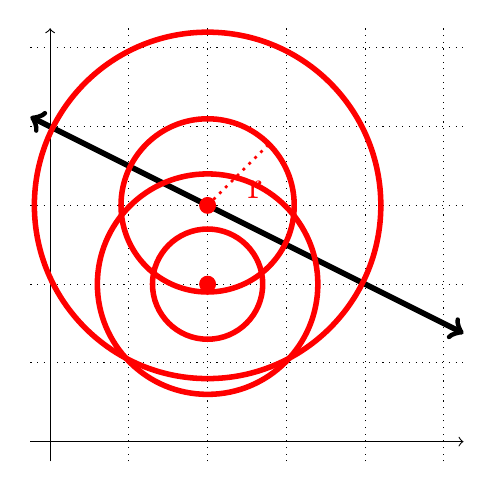
\begin{tikzpicture}[dot/.style={circle,inner sep=2pt,fill,name=#1},
    extended line/.style={shorten >=-#1,shorten <=-#1},
    extended line/.default=1cm]

% draw the grid
\draw[->] (0,-0.25) -- (0,5.25) ;
\draw[->] (-0.25,0) -- (5.25,0) ;
\foreach \i in {1,...,5} {
    \draw[dotted] (-0.25,\i) -- (5.25,\i);
    \draw[dotted] (\i,-0.25) -- (\i,5.25);
}

\uncover<2-3> {
    \draw[line width=2pt,<->] (-0.25,4.125) -- (5.25,1.375);
}

\uncover<1-2> {
    \node at (2.6,3.2) { \textcolor{red}{\Large r} };
    \path[draw=red,dotted,line width=1pt] (2,3) -- (2.8,3.8);
    \path[draw=red,fill=red] (2,3) circle (0.1);
    \path[draw=red,line width=2pt] (2,3) circle (1.1);
    \path[draw=red,line width=2pt] (2,3) circle (2.2);
}

\uncover<3> {
    %\node at (2.6,3.2) { \textcolor{red}{\Large r} };
    %\path[draw=red,dotted,line width=1pt] (2,2) -- (2.8,3.8);
    \path[draw=red,fill=red] (2,2) circle (0.1);
    \path[draw=red,line width=2pt] (2,2) circle (0.7);
    \path[draw=red,line width=2pt] (2,2) circle (1.4);
}

%\node[text width=8cm, align=left] at (10,3.5) {
    %\Large
%
%
    %%with the Euclidean distance.
%};


\end{tikzpicture}
}
&
\uncover<1> {
    \textbf{Example 1:}
    In the metric space $\mathbb{R}^2$,
    $$
    \cexp
    = \frac{\pi(2r)^2}{\pi r^2}
    = 4
    $$
    Define the \textbf{expansion dimension} as $\log_2 \cexp$.
    Then the expansion dimension of $\mathbb{R}^n$ is $O(n)$.
    %In general, the dimension of $\mathbb{R}^n$ is $O(n)$.
}
\\ &
\vspace{-1.5in}
\uncover<2> {
    \textbf{Example 2:}
    In the subspace of $\mathbb{R}^2$ given by
    $$
    %\mathcal{X} = \{ (x,y) : y = -0.5x+4 \}
    \{ (x,y) : y = -0.5x+4 \}
    $$
    we have
    $$
    \cexp
    = \frac{4r}{2r}
    = 2
    $$
    %So the dimensionality $\log_2 \cexp = 1$.
}
\\ &
\vspace{-1.75in}
\uncover<3> {
    \textbf{Example 3:}
    In the subspace of $\mathbb{R}^2$ given by
    $$
    %\mathcal{X} = \{ (x,y) : y = -0.5x+4 \}
    \{ (x,y) : y = -0.5x+4 \} \cup \{(2,2)\}
    $$
    we have
    $
    c
    %= \frac{\infty}{0}
    = \infty
    $
    %so the expansion dimension is also $\infty$.
}


\end{tabular}

\end{frame}
